\documentclass[11pt]{article}

\usepackage[a4paper,margin=1in]{geometry}
\usepackage{graphicx}
\usepackage{amsmath}
\usepackage{amssymb}
\usepackage{booktabs}
\usepackage{longtable}
\usepackage{float}
\usepackage{caption}
\usepackage[T1]{fontenc}
\usepackage[utf8]{inputenc}
\usepackage{textcomp}
\usepackage{hyperref}
\hypersetup{colorlinks=true,linkcolor=blue,urlcolor=blue}

% Layout for image grids
\newlength{\gridimg}
\setlength{\gridimg}{0.3\textwidth}

\graphicspath{{writeup_images/}}

\setlength{\parindent}{0pt}
\setlength{\parskip}{0.5em}

\title{Assignment 3: Diffusion Playground\\[0.3em]
\large Sampling, Editing, and Illusions with a Pretrained\\ Text-to-Image Diffusion Model (DeepFloyd IF)}
\author{Omer Yosef (207003187) \and Gal Barak (211699707)\\[0.4em]\normalsize Neural Graphics (3683-8901)}
\date{}

\begin{document}
\maketitle

\begin{quote}
\textbf{Note on images.} All figures are the outputs actually generated by
\texttt{Assignment3.ipynb} (the submitted notebook) and are stored in \texttt{./writeup\_images/}.
Results are stochastic and prompt-dependent; the exact prompts used are listed under
each task and summarised in the appendix.
\end{quote}

\hrulefill

\section*{Part 0: Loading the Model}

\subsection*{Task 0.1: Sampling with your own prompts + inference-step comparison}

\textbf{Prompts used (all exact keys in the precomputed embedding dictionary):}
\begin{itemize}
  \item \texttt{"an oil painting of an old man"}
  \item \texttt{"an oil painting of people around a campfire"}
  \item \texttt{"a rocket ship"}
\end{itemize}

\textbf{Random seed:} \texttt{100} (set with \texttt{seed\_everything(100)}, and reused for all later parts).

\textbf{Stage 1 (64$\times$64):}

\begin{figure}[H]
\centering

\includegraphics[width=\gridimg]{c16_0.png}\hfill

\includegraphics[width=\gridimg]{c16_1.png}\hfill

\includegraphics[width=\gridimg]{c16_2.png}
\caption*{old man / campfire / rocket ship --- stage 1}
\end{figure}

\textbf{Stage 2 (upsampled to 256$\times$256):}

\begin{figure}[H]
\centering
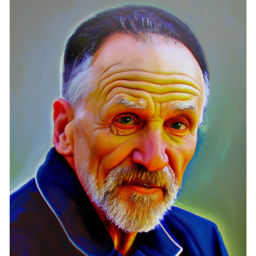
\includegraphics[width=\gridimg]{c16_3.png}\hfill
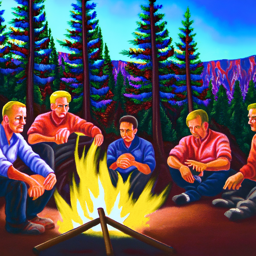
\includegraphics[width=\gridimg]{c16_4.png}\hfill
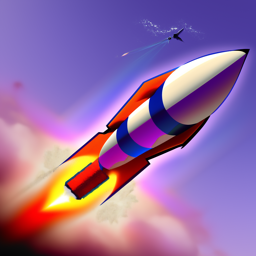
\includegraphics[width=\gridimg]{c16_5.png}
\caption*{old man / campfire / rocket ship --- stage 2}
\end{figure}

\textbf{Low vs.\ high \texttt{num\_inference\_steps}} (prompt \texttt{"a rocket ship"}):

\begin{figure}[H]
\centering
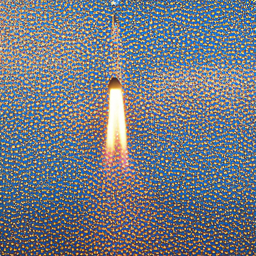
\includegraphics[width=\gridimg]{c16_6.png}\hspace{0.05\textwidth}
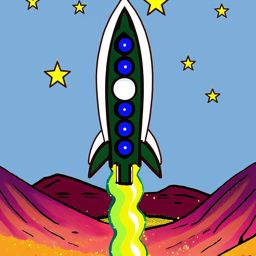
\includegraphics[width=\gridimg]{c16_7.png}
\caption*{5 steps (left) vs.\ 50 steps (right)}
\end{figure}

\textbf{Discussion.}
\begin{itemize}
  \item \emph{Stage 1 vs.\ Stage 2.} Stage 1 sets the overall composition and content at
  low resolution (64$\times$64); it looks right but soft. Stage 2 is a conditional
  super-resolution diffusion model that adds high-frequency detail (edges, texture) to
  reach 256$\times$256. The content stays the same, but the sharpness and fine structure
  improve a lot.
  \item \emph{5 vs.\ 50 steps.} With only 5 denoising steps the sampler can't remove the
  noise accurately, so the image is blurry, low-contrast, and hard to read. At 50 steps
  each reverse step is a smaller, more accurate update, which gives a sharp, coherent
  image. Most of the improvement happens by about 20 steps and then levels off; the
  50-step result is only a little better than a 20-step one despite costing much more.
\end{itemize}

\hrulefill

\section*{Part 1: Sampling-Loop Mechanics}

\subsection*{Task 1.1: The Forward Process}

The forward process adds noise per the pretrained schedule:
$x_t = \sqrt{\bar\alpha_t}\, x_0 + \sqrt{1-\bar\alpha_t}\,\varepsilon$,
$\varepsilon \sim \mathcal{N}(0, I)$. Test image noised at
$t \in \{250, 500, 750\}$:

\begin{figure}[H]
\centering

\includegraphics[width=0.23\textwidth]{c23_0.png}\hfill

\includegraphics[width=0.23\textwidth]{c23_1.png}\hfill

\includegraphics[width=0.23\textwidth]{c23_2.png}\hfill

\includegraphics[width=0.23\textwidth]{c23_3.png}
\caption*{original / $t=250$ / $t=500$ / $t=750$}
\end{figure}

\textbf{Discussion.} As $t$ grows, $\sqrt{\bar\alpha_t}$ shrinks and
$\sqrt{1-\bar\alpha_t}$ grows, so the clean signal is progressively drowned out by
Gaussian noise. At $t=250$ the structure is still clearly visible; by $t=750$ the image
is almost pure noise.

\subsection*{Task 1.2a: One-Step Denoising}

Using the UNet's noise estimate to jump straight to a clean-image estimate:
$\hat x_0 = (x_t - \sqrt{1-\bar\alpha_t}\,\hat\varepsilon_\theta(x_t, t)) / \sqrt{\bar\alpha_t}$.
Null prompt \texttt{"a high quality photo"}, at $t \in \{250, 500, 750\}$:

\begin{figure}[H]
\centering

\includegraphics[width=0.35\textwidth]{c25_0.png}
\caption*{original}
\end{figure}

\begin{table}[H]
\centering
\begin{tabular}{cc}
\toprule
noisy & one-step estimate \\
\midrule

\includegraphics[width=0.28\textwidth]{c25_1.png} & 
\includegraphics[width=0.28\textwidth]{c25_2.png} \\
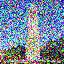
\includegraphics[width=0.28\textwidth]{c25_3.png} & 
\includegraphics[width=0.28\textwidth]{c25_4.png} \\

\includegraphics[width=0.28\textwidth]{c25_5.png} & 
\includegraphics[width=0.28\textwidth]{c25_6.png} \\
\bottomrule
\end{tabular}
\caption*{$t=250$ (top), $t=500$ (middle), $t=750$ (bottom)}
\end{table}

\textbf{Discussion.} The one-step estimate is good at low noise ($t=250$) but degrades
badly as $t$ rises: at $t=750$ it is blurry and washed out, because the model must
reconstruct the entire clean image from almost pure noise in a single shot.

\subsection*{Task 1.2b: Iterative Denoising (strided schedule)}

\texttt{strided\_timesteps = list(range(990, -1, -30))} $\rightarrow$ \textbf{34 timesteps}
(990, 960, \ldots, 30, 0), following the DDPM reverse step
\[
x_{t'} = \frac{\sqrt{\bar\alpha_{t'}}\,\beta_t}{1-\bar\alpha_t}\,\hat x_0
       + \frac{\sqrt{\alpha_t}\,(1-\bar\alpha_{t'})}{1-\bar\alpha_t}\,x_t
       + \sigma_t z,
\]
with $\alpha_t = \bar\alpha_t/\bar\alpha_{t'}$, $\beta_t = 1-\alpha_t$. The iterative loop
was run starting from a test image noised to \texttt{i\_start = 10}.

\subsection*{Task 1.2c: One-Step vs.\ Iterative (same noise level, \texttt{i\_start = 10})}

\begin{figure}[H]
\centering
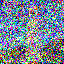
\includegraphics[width=\gridimg]{c31_0.png}\hfill

\includegraphics[width=\gridimg]{c31_1.png}\hfill

\includegraphics[width=\gridimg]{c31_2.png}
\caption*{noisy (i\_start=10) / iterative / one-step}
\end{figure}

\textbf{Discussion: why iterative denoising beats one-step with the same model.}
Look at the rightmost panel above: the one-step result is a smeared, ghostly campanile,
while the iterative one in the middle is crisp. Here is how we read it. At this noise
level many different clean images could have produced the same noisy $x_t$, and the UNet
only gets to output a single noise guess, so its one-shot answer lands on something like
the average of all of them, which is exactly why $c31\_2$ looks washed out. The iterative
version instead peels off a little noise per step; after each step the image is slightly
cleaner, fewer clean images are still consistent with it, and the model can commit to one
of them and start filling in real detail. Same weights in both runs, so all of the gain
comes from splitting the work into many small, easy steps rather than one big leap.

\subsection*{Task 1.3: Sampling With and Without CFG}

Prompt \texttt{"a high quality photo"}; CFG uses
$\varepsilon_{\text{cfg}} = \varepsilon_u + \gamma(\varepsilon_c - \varepsilon_u)$ with
$\gamma = 7$.

\textbf{Without CFG (5 samples):}

\begin{figure}[H]
\centering
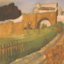
\includegraphics[width=0.185\textwidth]{c33_0.png}\hfill
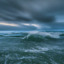
\includegraphics[width=0.185\textwidth]{c33_1.png}\hfill

\includegraphics[width=0.185\textwidth]{c33_2.png}\hfill
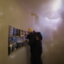
\includegraphics[width=0.185\textwidth]{c33_3.png}\hfill
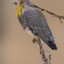
\includegraphics[width=0.185\textwidth]{c33_4.png}
\end{figure}

\textbf{With CFG, $\gamma = 7$ (5 samples):}

\begin{figure}[H]
\centering

\includegraphics[width=0.185\textwidth]{c33_5.png}\hfill

\includegraphics[width=0.185\textwidth]{c33_6.png}\hfill

\includegraphics[width=0.185\textwidth]{c33_7.png}\hfill

\includegraphics[width=0.185\textwidth]{c33_8.png}\hfill

\includegraphics[width=0.185\textwidth]{c33_9.png}
\end{figure}

\textbf{Discussion.} The top row (no CFG) is pretty underwhelming: dull, low-contrast,
and a couple of them barely look like photos at all. The bottom row with $\gamma=7$ is a
clear step up: sharper, more saturated, and much more convincingly photographic, which
makes sense because guidance pushes away from the unconditional estimate and leans harder
into the conditional one. The cost shows up in variety: our five CFG samples resemble each
other more than the five un-guided ones do.

\hrulefill

\section*{Part 2: Image Editing}

\subsection*{Task 2.1: SDEdit on the provided image and on your own image}

Procedure: noise the input to the timestep for each
\texttt{i\_start} $\in \{1, 3, 5, 7, 10, 20\}$, then run \texttt{iterative\_denoise\_cfg}
from that point with the null prompt \texttt{"a high quality photo"}.

\textbf{Provided test image (campanile):}

\begin{figure}[H]
\centering

\includegraphics[width=0.23\textwidth]{c36_0.png}\hfill
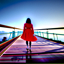
\includegraphics[width=0.23\textwidth]{c36_1.png}\hfill
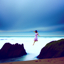
\includegraphics[width=0.23\textwidth]{c36_2.png}\hfill

\includegraphics[width=0.23\textwidth]{c36_3.png}\\[0.4em]

\includegraphics[width=0.23\textwidth]{c36_4.png}\hfill

\includegraphics[width=0.23\textwidth]{c36_5.png}\hfill

\includegraphics[width=0.23\textwidth]{c36_6.png}
\caption*{original / i\_start = 1, 3, 5, 7, 10, 20}
\end{figure}

\textbf{Own image, web image} (source: a downloaded web image):

\begin{figure}[H]
\centering

\includegraphics[width=0.3\textwidth]{c39_0.png}
\caption*{web source}
\end{figure}

\begin{figure}[H]
\centering

\includegraphics[width=0.3\textwidth]{c40_0.png}\hfill

\includegraphics[width=0.3\textwidth]{c40_1.png}\hfill

\includegraphics[width=0.3\textwidth]{c40_2.png}\\[0.4em]

\includegraphics[width=0.3\textwidth]{c40_3.png}\hfill

\includegraphics[width=0.3\textwidth]{c40_4.png}\hfill

\includegraphics[width=0.3\textwidth]{c40_5.png}
\caption*{i\_start = 1, 3, 5, 7, 10, 20}
\end{figure}

\textbf{Own image, hand-drawn:}

\begin{figure}[H]
\centering
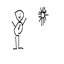
\includegraphics[width=0.3\textwidth]{c41_0.png}
\caption*{hand-drawn source}
\end{figure}

\begin{figure}[H]
\centering

\includegraphics[width=0.3\textwidth]{c42_0.png}\hfill

\includegraphics[width=0.3\textwidth]{c42_1.png}\hfill
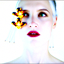
\includegraphics[width=0.3\textwidth]{c42_2.png}\\[0.4em]

\includegraphics[width=0.3\textwidth]{c42_3.png}\hfill
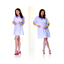
\includegraphics[width=0.3\textwidth]{c42_4.png}\hfill
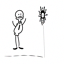
\includegraphics[width=0.3\textwidth]{c42_5.png}
\caption*{i\_start = 1, 3, 5, 7, 10, 20}
\end{figure}

\textbf{Discussion: edit strength vs.\ \texttt{i\_start}.} \texttt{i\_start} controls how
much noise we add before denoising again, i.e.\ how far back in the schedule we jump in.
You can watch the effect march across the panels: at \texttt{i\_start}$=1$ the output is
almost the input untouched, since we barely disturbed it; by \texttt{i\_start}$=5$--$7$ the
model is clearly repainting things while the overall layout survives; and at
\texttt{i\_start}$=20$ so much of the original signal is gone that the model reinvents big
chunks and the result wanders well away from what we fed it. So low \texttt{i\_start} keeps
you faithful and high \texttt{i\_start} lets the model get creative. This was most fun to
watch on the hand-drawn input, which only really starts to look like a real photo once we
push \texttt{i\_start} up to the higher values.

\subsection*{Task 2.2: Inpainting}

New content is generated only inside a binary mask (1 = regenerate); everything outside is
forced back to the original image, re-noised to the current timestep, at every step.

\textbf{Provided test image (mask over a region):}

\begin{figure}[H]
\centering

\includegraphics[width=0.3\textwidth]{c44_0.png}\hfill

\includegraphics[width=0.3\textwidth]{c44_1.png}\hfill

\includegraphics[width=0.3\textwidth]{c44_2.png}
\caption*{image / mask / to replace}
\end{figure}

\begin{figure}[H]
\centering

\includegraphics[width=0.3\textwidth]{c45_0.png}\hfill

\includegraphics[width=0.3\textwidth]{c45_1.png}\hfill

\includegraphics[width=0.3\textwidth]{c45_2.png}
\caption*{original / mask / inpainted}
\end{figure}

\textbf{Own image, own mask} (inpainting the web image with a custom rectangular mask):

\begin{figure}[H]
\centering

\includegraphics[width=0.3\textwidth]{c46_0.png}\hfill

\includegraphics[width=0.3\textwidth]{c46_1.png}\hfill

\includegraphics[width=0.3\textwidth]{c46_2.png}
\caption*{original / mask / inpainted}
\end{figure}

\textbf{Discussion.} The reverse process runs normally inside the mask, but at each step
the region outside the mask is overwritten with the original image noised to match the
current timestep. This keeps the surroundings fixed while letting the model generate new,
context-consistent content inside the masked region. The boundary stays coherent because
the model always sees the true (re-noised) surroundings while it denoises.

\subsection*{Task 2.3: Text-Conditioned Image-to-Image Translation}

Same as SDEdit but steered by a real prompt instead of the null prompt.
\textbf{Prompt used: \texttt{"a rocket ship"}}, \texttt{i\_start} $\in \{1, 3, 5, 7, 10, 20\}$
on the provided test image.

\begin{figure}[H]
\centering
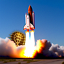
\includegraphics[width=0.3\textwidth]{c48_0.png}\hfill

\includegraphics[width=0.3\textwidth]{c48_1.png}\hfill

\includegraphics[width=0.3\textwidth]{c48_2.png}\\[0.4em]

\includegraphics[width=0.3\textwidth]{c48_3.png}\hfill
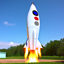
\includegraphics[width=0.3\textwidth]{c48_4.png}\hfill
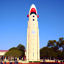
\includegraphics[width=0.3\textwidth]{c48_5.png}
\caption*{i\_start = 1, 3, 5, 7, 10, 20}
\end{figure}

\textbf{Discussion.} Compared with the null-prompt edit in Task 2.1, the text prompt
injects \emph{semantic} content, not just ``realism.'' At low \texttt{i\_start} the tall
campanile silhouette is preserved but nudged toward rocket-like features; at high
\texttt{i\_start} the model is free enough to reshape the image into an actual rocket ship.
The prompt controls which kind of real image the result is pulled toward, so the chosen
words change what the edit becomes, not just how strong it is.

\hrulefill

\section*{Part 3: Diffusion Illusions}

\subsection*{Task 3.1: Visual Anagrams}

Combined noise estimate
$\varepsilon = \tfrac{1}{2}\big(\varepsilon_\theta(x_t, t, p_1) + \text{flip}(\varepsilon_\theta(\text{flip}(x_t), t, p_2))\big)$,
$\gamma = 7$, denoised from pure noise (\texttt{i\_start = 0}).

\begin{itemize}
  \item $p_1$ (upright) $=$ \texttt{"an oil painting of an old man"}
  \item $p_2$ (flipped) $=$ \texttt{"an oil painting of people around a campfire"}
\end{itemize}

\begin{figure}[H]
\centering

\includegraphics[width=0.35\textwidth]{c50_0.png}\hspace{0.05\textwidth}

\includegraphics[width=0.35\textwidth]{c50_1.png}
\caption*{upright: an old man / flipped: people around a campfire}
\end{figure}

\textbf{Discussion.} Because the two noise estimates are averaged (one on the image, one on
its vertical flip), the reverse process is simultaneously pulled toward both prompts under
their respective orientations. The result reads as an old man right-side up and as people
around a campfire when flipped.

\subsection*{Task 3.2: Hybrid Images (Bonus)}

Combined estimate
$\varepsilon = f_{\text{low}}(\varepsilon_\theta(x_t, t, p_{\text{low}})) + f_{\text{high}}(\varepsilon_\theta(x_t, t, p_{\text{high}}))$,
where $f_{\text{low}}$ is a Gaussian blur (\texttt{kernel\_size=9}, \texttt{sigma=2.0}) and
$f_{\text{high}}$ is the estimate minus its own low-pass. $\gamma = 7$, \texttt{i\_start = 0}.

\begin{itemize}
  \item $p_{\text{low}}$ (low frequencies / far) $=$ \texttt{"a lithograph of waterfalls"}
  \item $p_{\text{high}}$ (high frequencies / near) $=$ \texttt{"a lithograph of a skull"}
\end{itemize}

\begin{figure}[H]
\centering
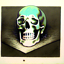
\includegraphics[width=0.35\textwidth]{c52_0.png}
\caption*{hybrid (far: waterfalls / near: skull)}
\end{figure}

\textbf{Upsampled to 256$\times$256} (optional stage-2 pass):

\begin{figure}[H]
\centering
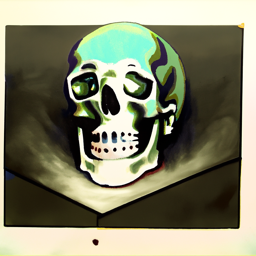
\includegraphics[width=0.35\textwidth]{c54_0.png}
\caption*{hybrid upsampled}
\end{figure}

\textbf{Discussion: which prompt dominates far vs.\ near, and why.} The \textbf{waterfalls}
prompt wins \emph{from a distance}, because it provides the low spatial frequencies that set
the overall shape and layout, and our eyes rely more on low frequencies when an image is
small or blurry. The \textbf{skull} prompt wins \emph{up close}, because it provides the high
frequencies (fine texture and edges) that we only pick out at short range. Applying the
low-pass/high-pass split to the \emph{noise estimate} instead of to the pixels makes the model
build this split directly into the generated image, so one picture reads as two different
subjects depending on how far away you are. It works best when the two subjects have a similar
rough outline, so the low-frequency prompt sets the shape and the high-frequency prompt just
adds texture on top.

\hrulefill

\section*{Appendix: Prompts and Parameters Used}

\begin{longtable}{p{0.08\textwidth} p{0.45\textwidth} p{0.37\textwidth}}
\toprule
\textbf{Task} & \textbf{Prompt(s)} & \textbf{Key parameters} \\
\midrule
\endhead
0.1 & old man / campfire / rocket ship & stage 1 \& 2 \texttt{num\_inference\_steps=20}; comparison 5 vs 50 (rocket) \\
1.1 & n/a & $t \in \{250, 500, 750\}$ \\
1.2a & \texttt{"a high quality photo"} (null) & $t \in \{250, 500, 750\}$ \\
1.2b & \texttt{"a high quality photo"} & \texttt{strided\_timesteps = range(990,-1,-30)} (34 steps), \texttt{i\_start=10} \\
1.2c & \texttt{"a high quality photo"} & \texttt{i\_start=10} (one-step vs iterative) \\
1.3 & \texttt{"a high quality photo"} & 5 samples no-CFG + 5 samples CFG, $\gamma=7$ \\
2.1 & \texttt{"a high quality photo"} (null) & \texttt{i\_start} $\in \{1,3,5,7,10,20\}$; campanile + web + hand-drawn \\
2.2 & \texttt{"a high quality photo"} & provided mask (campanile) + custom mask on web image \\
2.3 & \texttt{"a rocket ship"} & \texttt{i\_start} $\in \{1,3,5,7,10,20\}$ \\
3.1 & \texttt{"an oil painting of an old man"} / \texttt{"an oil painting of people around a campfire"} & $\gamma=7$, \texttt{i\_start=0} \\
3.2 & \texttt{"a lithograph of waterfalls"} (low) / \texttt{"a lithograph of a skull"} (high) & Gaussian blur k=9, $\sigma=2.0$; $\gamma=7$, \texttt{i\_start=0} \\
\bottomrule
\end{longtable}

\textbf{CFG guidance scale used throughout Parts 2--3:} $\gamma = 7$.

\end{document}
